\documentclass[a4paper,]{article}
\usepackage[left=2.5cm,top=2.5cm,right=2.5cm,bottom=3cm]{geometry} 
\usepackage[utf8]{inputenc}
\usepackage{graphicx} % Required for inserting images
\usepackage[table,xcdraw]{xcolor}
\usepackage{lipsum} % for dummy text
\usepackage{mathdots} % para el comando \iddots
\usepackage{mathrsfs} % para formato de letra
\usepackage{marvosym}
\usepackage{amsmath}
\usepackage{amsfonts}
\usepackage{amssymb}
\usepackage{listings}
\usepackage{caption}
\usepackage{float}


\title{\textbf{HW1: Introduction to Financial Engineering} \\ Time series}
\author{Miguel Angel Aguilo Gonzalez, 1699413 \\ Judit de Paz Ramírez, 1570590 \\ Laia Mòdol Rodríguez, 1565282 \\ Elena Rubio Zabala, 1699049 \\ Guillem Tutusaus Alcaraz, 1533701 } 
\date{Octubre 2023}

\begin{document}

\maketitle
\newpage

\section*{Ejercicio 1}
Dada una serie temporal, decimos que un proceso es estacionario si después de un tiempo sus propiedades como media, varianza y covarianza no han cambiado. \\

Un proceso estacionario muestra oscilaciones alrededor del mismo nivel de reversión a la media; para cualquier dato real, uno puede adivinar simplemente mediante el gráfico cuáles de ellos no son estacionarios y realizando una prueba adecuada para justificar cuáles lo son. Vamos a estudiar el caso de la serie temporal de los datos extraídos de "The 91-day treasury bill" (r), "The log of real GPD" (y) y "The inflation Rate" (pi).\\

Para realizar el estudio, consideremos sus gráficos:
\begin{figure}[h!]
    \centering
    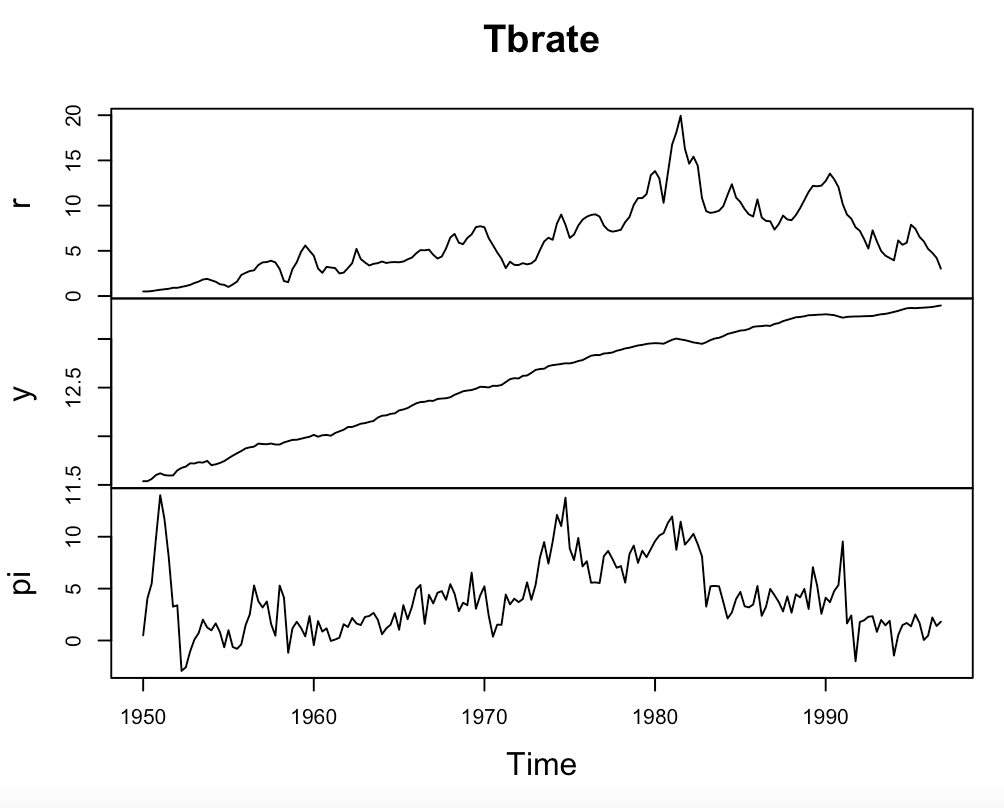
\includegraphics[scale=0.65]{t_series_plot.png}
\end{figure}


Podemos ver que la gráfica de "r", muestra varias características  estacionarias a pesar de su enorme volatilidad. En cambio, las gráficas de "y" y "pi" tenen una tendencia positiva, lo que significa que es casi seguro que "r" e "y" no sean procesos estacionarios.


\vspace{5mm}


Ahora, observemos los gráficos ACF:

\begin{figure}[h!]
    \centering
    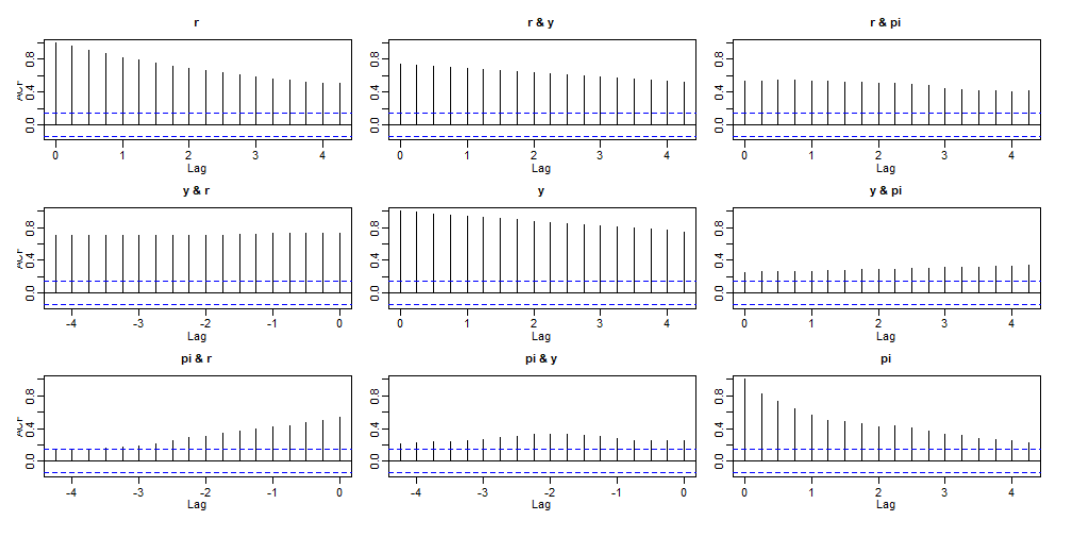
\includegraphics[scale=0.65]{ACF.png}
\end{figure}

Observemos los gráficos de "r","y" y "pi". En primer lugar, dado que casi todos los gráficos muestran retrasos distintos de cero, está claro que no son un ruido blanco, lo que significa que no son aleatorios. Podemos notar que no hay retraso donde el ACF caiga drasticamente, lo que nos indica que no se trata de MA(q). También, al ver que su caída no es exponencial podemos descartar la idea de que sea un modelo AR(p). Los gráficos ACF de "r", "y" y "pi" muestran una lenta caída a cero, esto es un signo de una memoria de dependencia prolongada o de un proceso no estacionario.\\

A parte de las observaciones de los gráficos que presentan una tendencia a modelos no estacionarios, realizaremos con R el Dickey-Fuller Test.\\

Sabemos que un modelo $ARMA(p,q)$ tiene la forma:
$$ Y_t-\mu= \sum_{i=1}^{p}\phi_i(Y_{t-i}-\mu)+\epsilon_t+\sum_{j=1}^{q}\delta_j\epsilon_{t-q} $$
éste es estacionario si las raices del polinomio $1-\sum_{i=1}^{p}\phi_ix^i$ tienen valor absoluto mayor que uno. \\

La Prueba de Dickey-Fuller busca determinar la existencia o no de raíces unitarias en una serie temporal. La hipótesis nula de esta prueba es que existe una raíz unitaria en la serie. Los resultados incluyen estadísticas de la prueba, el p-valor. Sabemos que si este valor es menor que un nivel de significancia dado (0,05), podemos rechazar la hipótesis nula. El Lag order es el número de retardos utilizados en la regresión del ADF.
\begin{lstlisting}[language=R]
> adf.test(Tbrate[,1]) 
p-value = 0.6075
alternative hypothesis: stationary

> adf.test(Tbrate[,2])
p-value = 0.9873
alternative hypothesis: stationary

> adf.test(Tbrate[,3])
p-value = 0.1788
alternative hypothesis: stationary
\end{lstlisting}

% \begin{figure}[h!]
   % \centering
   % 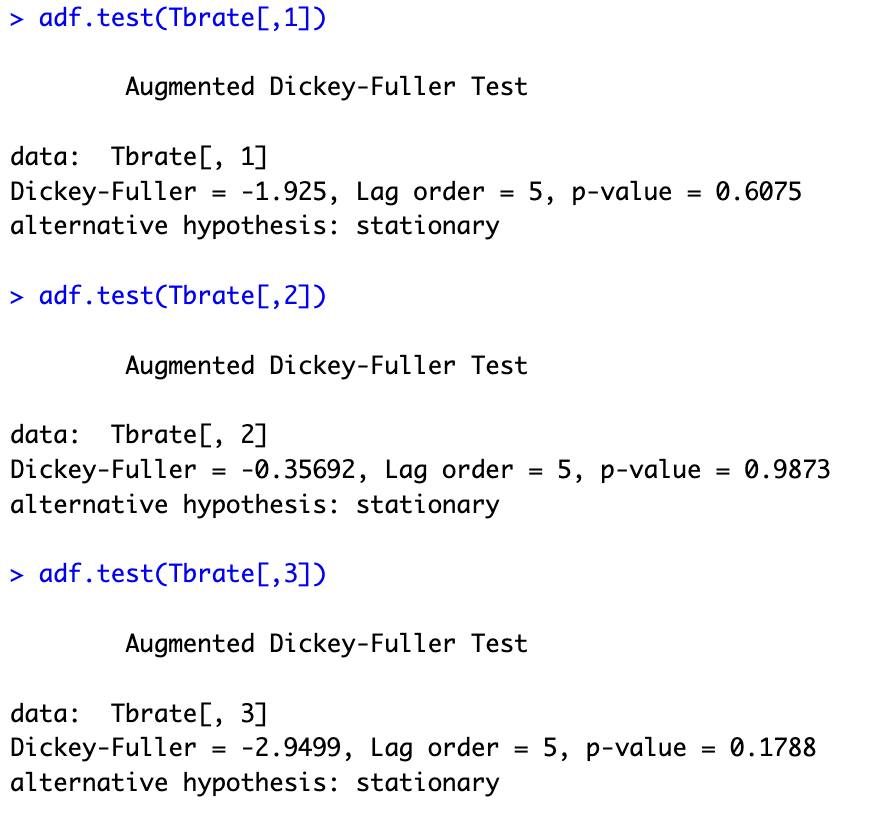
\includegraphics[scale=0.65]{dickey.png}
% \end{figure}

No podemos rechazar la hipótesis nula porque el p-valor no es menor que 0,05 en ninguno de los casos. Por lo tanto, aceptamos la hipótesis nula, es decir, existe una raíz unitaria en la serie y por lo tanto presenta un modelo no estacionario.\\
A pesar de los resultados, estudiamos ahora las series temporales transformadas para ver si se pueden modelar como un proceso $ARMA(p,q)$. \\

Esta vez la prueba de Dickey-Fuller nos da un p-valor menor que 0,01 en los tres casos. Como el p-valor es menor que 0,05 rechazamos la hipotesis nula (nos dice que la serie temporal tiene una raíz unitaria y por lo tanto no es estacionaria) y nos quedamos con la hipótesis alternativa concluyendo que la serie es estacionaria para todas las variables.\\

% Observemos el resultado:

% \begin{figure}[h!]
  %  \centering
   % 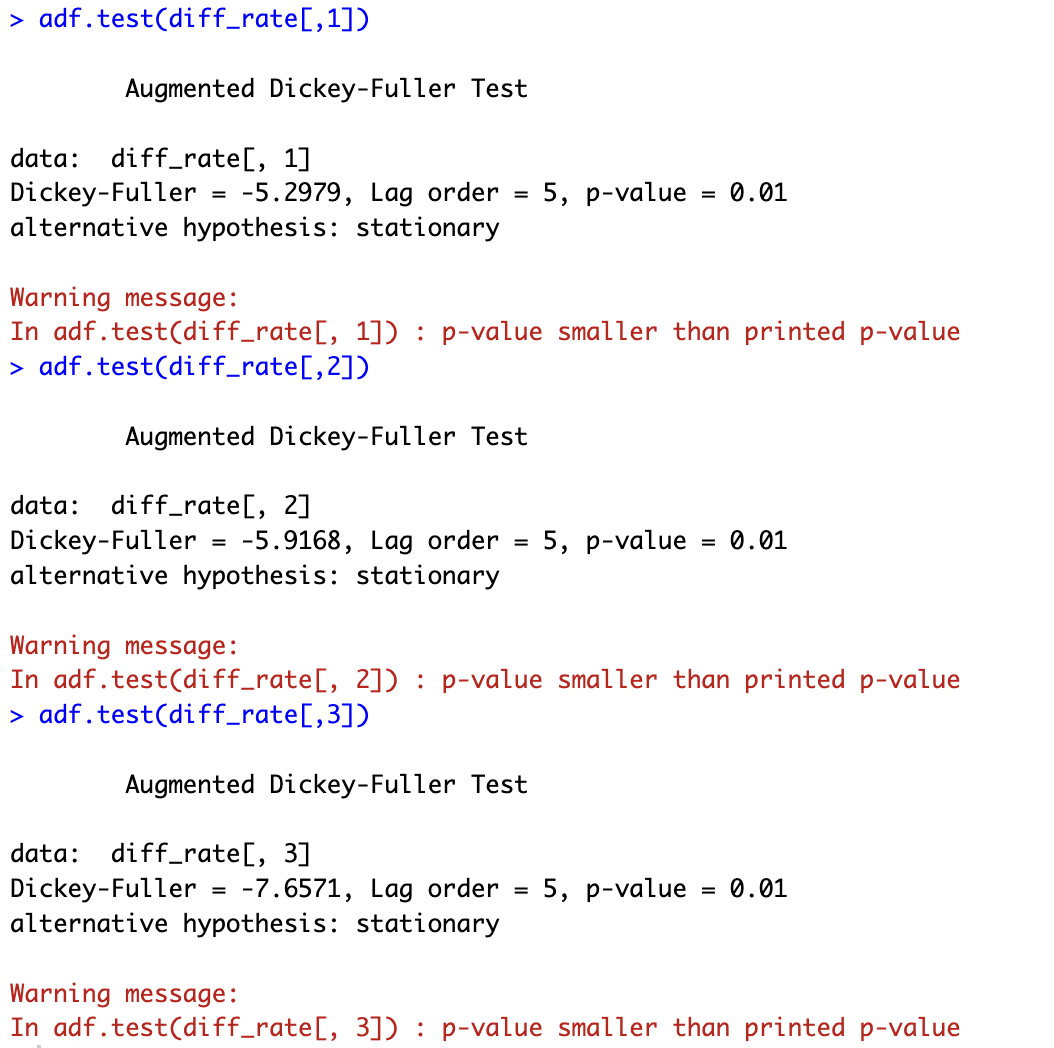
\includegraphics[scale=0.65]{diff_dickey.png}
%\end{figure}

Viendo los gráficos de la serie temporal transformada vemos que la correlación entre lags muestra en general autocorrelaciones de valores entre 0 y 0,05, lo que significa que no son aleatorios, un modelo ARMA(p,q) es el más adecuado para ellos.\\

\begin{figure}[H]
    \centering
    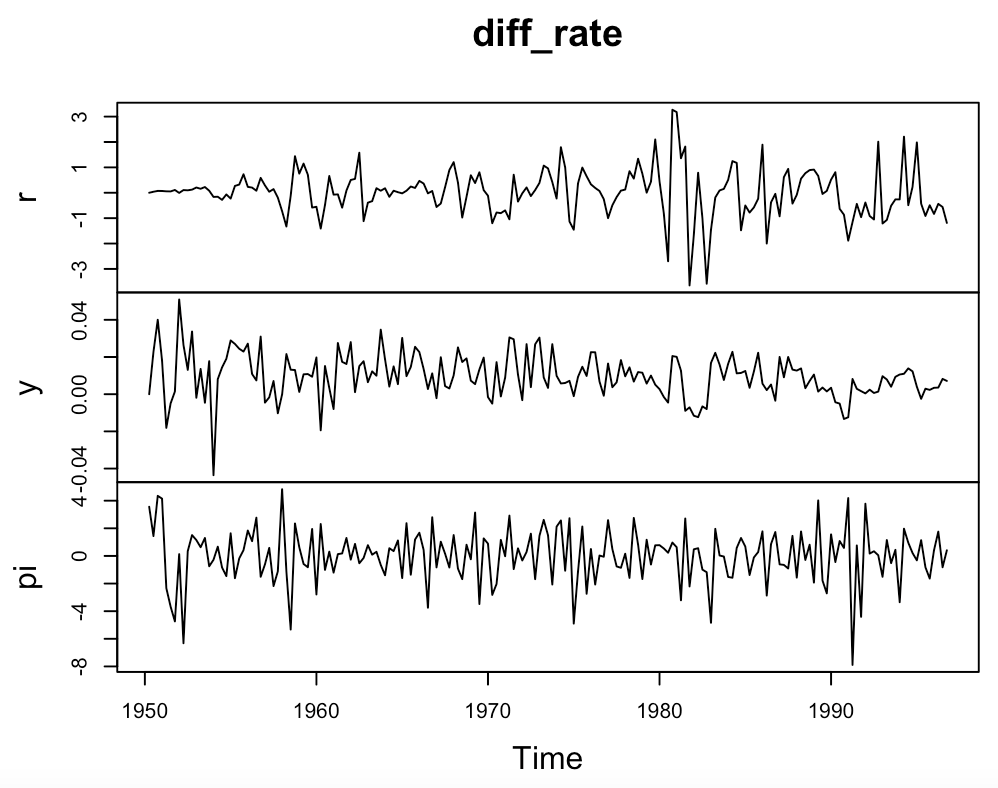
\includegraphics[scale=0.4]{dif_rate.png}
    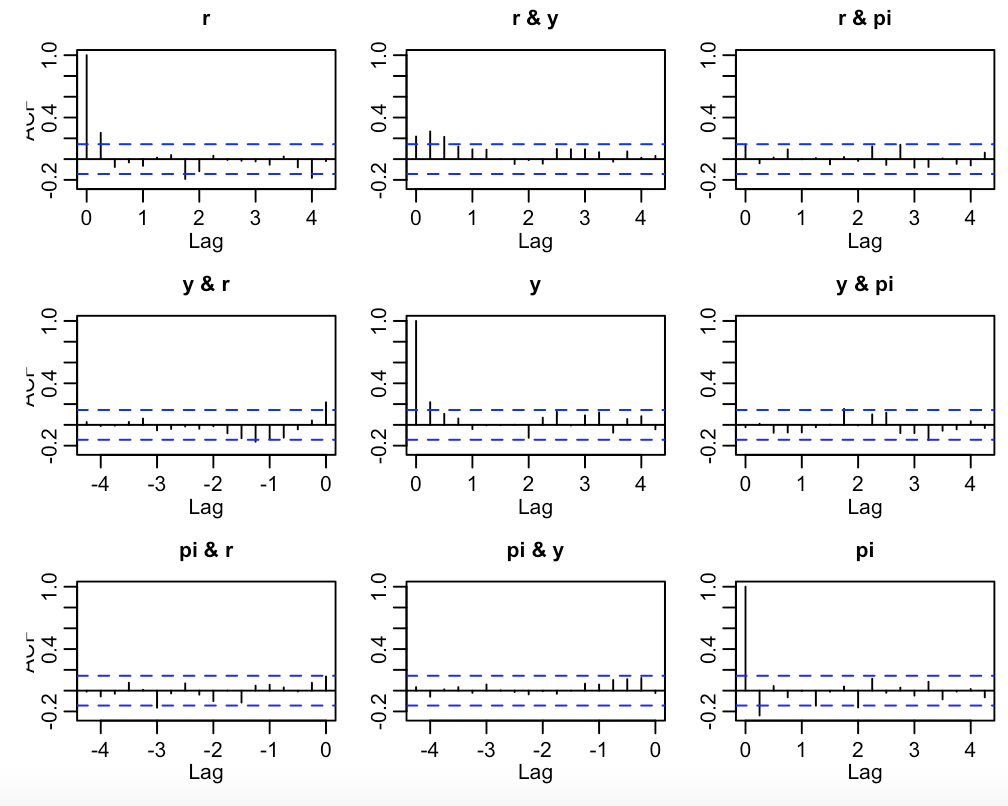
\includegraphics[scale=0.4]{diff_acf.png}
    \caption*{Gráficos de la serie temporal transformada}
\end{figure}

En particular, los gráficos de ACF comparten que después de un retraso el AFC es significativamente 0 y sus colas parecen estrechas.\\

Se observa que los gráficos no presentan tendencias no estacionarias.\\

En conclusión, parecen comportarse como ARIMA(0,1,1) según los gráficos ACF.\\

\bigskip
Veamos el modelo de mejor ajuste obtenido por \texttt{auto.arima()}, la función incorporada de R que proporciona esta respuesta, con AIC (Akaike Information Criterion): \\
%\begin{figure}[h!]
 %   \centering
  %  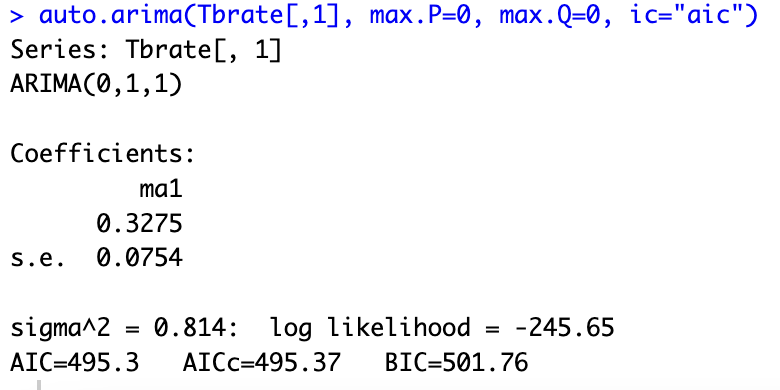
\includegraphics[scale=0.5]{auto.arima1.png}
%\end{figure}

\begin{lstlisting}[language=R]
> auto.arima(Tbrate[,1], max.P=0, max.Q=0, ic="aic")
Series: Tbrate[, 1] 
ARIMA(0,1,1) 

Coefficients:
         ma1
      0.3275
s.e.  0.0754

sigma^2 = 0.814:  log likelihood = -245.65
AIC=495.3   AICc=495.37   BIC=501.76
\end{lstlisting}

Observamos también que el AIC eligió el modelo ma(1). Los dos criterios de bondad más comunes para esta función son el AIC y el BIC,  Cuanto menor sea el valor de AIC, mejor se considera el modelo. El AIC penaliza menos la complejidad del modelo en comparación con el BIC, lo que significa que puede seleccionar modelos más complejos si proporcionan un mejor ajuste a los datos. De esta manera, el criterio de bondad de ajuste que usamos aquí será e AIC más pequeño.\\

Cuando cambiamos el criterio de bondad a BIC
 %\begin{figure}[h!]
  %  \centering
  %  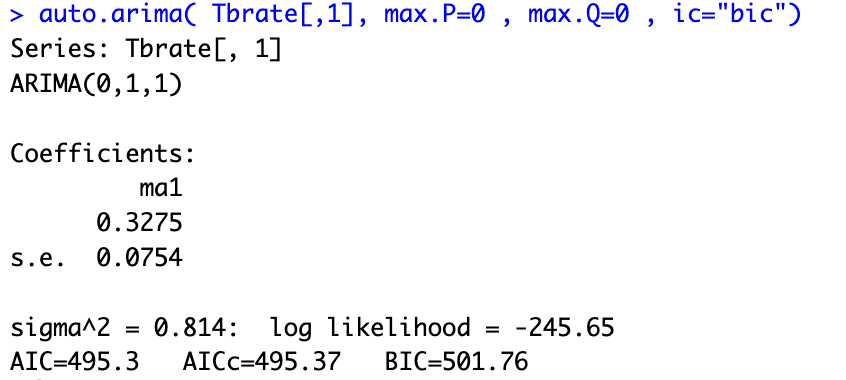
\includegraphics[scale=0.5]{auto.arima2.png}
%\end{figure}
nos damos cuenta que no cambia el modelo que más se ajusta ya que sigue eligiendo el modelo ma(1).\\

En particular, el orden de diferenciación elegido es 1 y ese es el mismo orden que obtuvimos del análisis anterior para esos datos. \\

Podemos ver que el gráfico ACF de residuos no muestra autocorrelación residual. 
\begin{figure}[H]
    \centering
    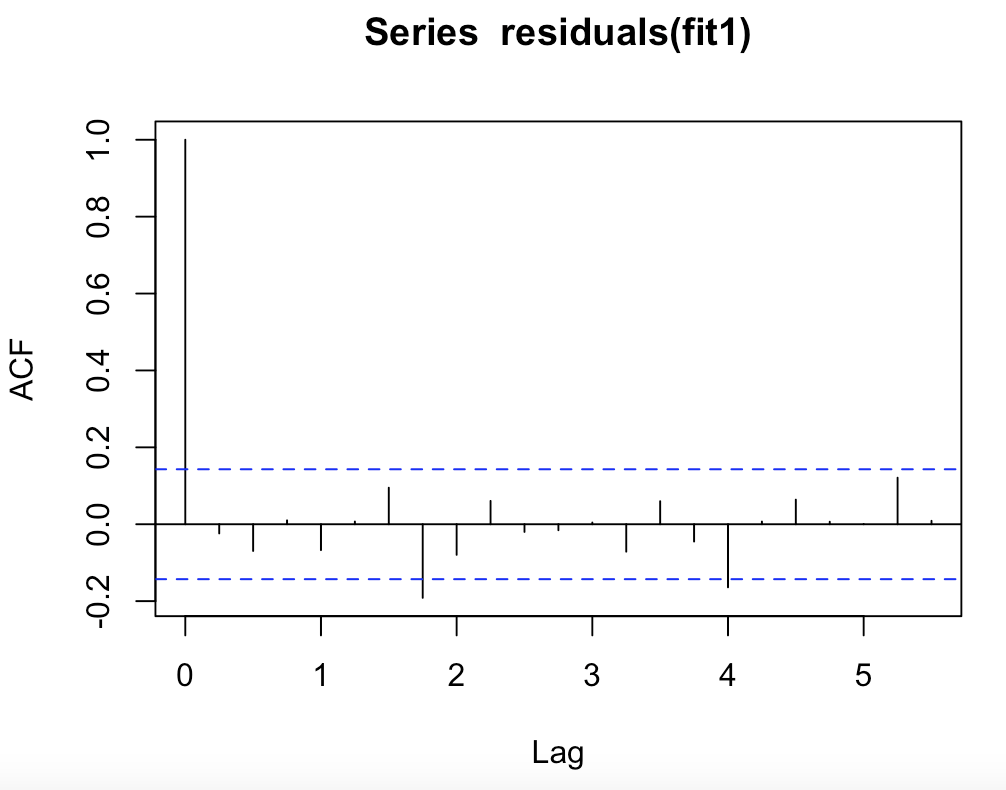
\includegraphics[scale=0.5]{residuals.png}
    \caption*{Gráfico ACF de los residuos}
\end{figure}
Además, haremos un Box-test, el cual nos dice que aceptemos la hipótesis nula: los residuos son independientes entre sí:
\begin{lstlisting}[language=R]
> Box.test(residuals(fit1),lag=10,type="Ljung")

	Box-Ljung test

data:  residuals(fit1)
X-squared = 13.017, df = 10, p-value = 0.2227
\end{lstlisting}

%\begin{figure}[h!]
%    \centering
 %   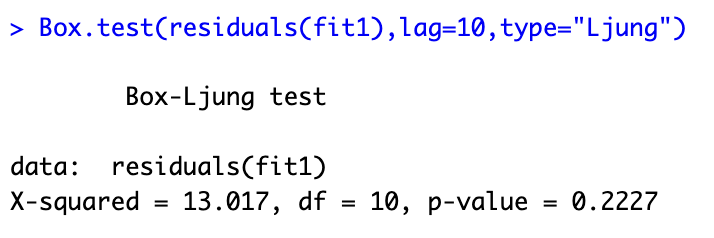
\includegraphics[scale=0.5]{box.png}
%\end{figure}


Es decir no queda información en los residuos de la serie temporal original, lo cual nos indica que el modelo propuesto es bastante bueno para pronosticar valores de futuros y dar predicciones.\\


\section*{Ejercicio 2}
Sea $\{\varepsilon\}_n$ un $WN(0, \sigma^2)$. Decimos que $\{Y_n\}_n$ es un proceso $AR(1)$ si para algún parámetro constante $\mu$ y $\phi$, se cumple la siguiente ecuación: $$Y_t-\mu=\phi(Y_{t-1}-\mu)+\varepsilon_t$$
\\

El parámetro $\mu$ es la media del proceso y el término $\phi(Y_{t-1}-\mu)$ representa la memoria, en particular la constante $\phi$ determina la velocidad de la reversión a la media del proceso. Observamos que para que $Y$ sea un proceso débilmente estacionario necesitamos $|\phi|<1$. Para derivar esta observación, llamamos $\sigma_Y$ a la varianza de $Y_t$, que por independencia, sigue $$\sigma_Y^2=\phi^2\sigma_Y^2+\sigma_\varepsilon^2.$$
\\
Consideremos el siguente modelo AR $$Y_t=5-0,55Y_{t-1}+\varepsilon_t$$ asumiendo $\sigma_\varepsilon^2=1,2.$ \\

Usando la primera fórmula nos damos cuenta de que $\phi=-0,55$, por lo tanto, $|\phi|=|-0,55|=0,55<1$, de esta forma podemos ver que es un modelo estacionario. Al ser un modelo estacionario podemos determinar fácilmente los estadísticos de la media, la varianza y la función de covarianza.
\begin{align*}
    \mathbb{E}[Y_t]&=\mu=\frac{5}{1-\phi}=3,225806 \\
    \gamma(0)&=\mathbb{V}[Y_t]=\frac{\sigma_\epsilon^2}{1-\phi^2}=\frac{(1,2)^2}{1-(-0,55)^2}=1,72043 \\
    \gamma(i-j)&=Cov(Y_i,Y_j)=\frac{\sigma_\epsilon^2}{1-\phi^2} \phi^{|i-j|}=1,72043 \cdot (-0,55)^{|i-j|}
\end{align*}

\section*{Ejercicio 3}
Un modelo AR(3) tiene la forma siguiente:
 $$Y_{t+1} - \mu = \phi_{1}(Y_t - \mu) + \phi_{2}(Y_{t-1} -\mu) + \phi_{3}(Y_{t-2} -\mu) + \varepsilon_{t+1}$$ donde $\mu, \phi_{1},\phi_{2} $ y $ \phi_{3} $ son constantes y $\varepsilon_{t+1}$ es un $WN(0, \sigma^2)$.\\

Conociendo los valores de $Y_{1},Y_{2},...,Y_{t}$ , los parámetros $\phi_{1},\phi_{2} $ y $ \phi_{3} $ y usando la estimación para la media $\hat{\mu}$ nos gustaría preveer los valores $Y_{t+1}$ y $Y_{t+2}$.\\

Para ello, aunque no sepamos el valor de $\varepsilon_{t+1}$, como es independiente de las $\{Y_{i}\}_i$  podemos usar que su media es 0 como la mejor aproximación. Por lo que, conseguiriamos esta fórmula de predicción para calcular los valores que buscamos: 

 $$\hat{Y_{t+1}} = \hat{\mu}  + \phi_{1}(Y_t - \hat{\mu}) + \phi_{2}(Y_{t-1} -\hat{\mu}) + \phi_{3}(Y_{t-2} -\hat{\mu}).$$

 En nuestro caso, $\mu=104 $ , $\phi_{1} =0.4 $ , $\phi_{2}=0.25 $ , $\phi_{3} =0.1$, $Y_{t}=99$, $Y_{t-1}=103$ y $Y_{t-2}=102$
 Sustituyendo los valores en la fórmula conseguimos que $Y_{t+1}=101.55$ y utilizando éste conseguimos $Y_{t+2}= 101.67$.\\
 
\section*{Ejercicio 4}
Hacemos primero el gráfico de la serie temporal del índice americano de precios desde 1950 a 1990 y el gráfico ACF para determinar cuántas veces tenemos que transformar la función para obtener un proceso estacionario.

\begin{figure}[H]
    \centering
    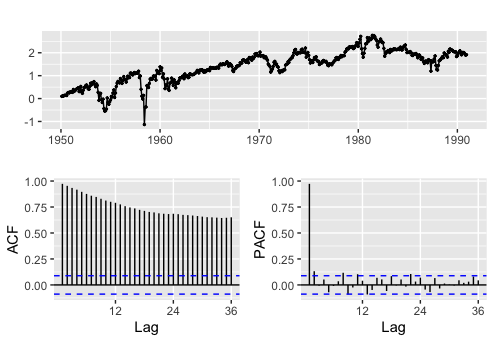
\includegraphics[width=0.7\linewidth]{mishkin1.png}
\end{figure}


Vemos que la serie presenta una tendencia creciente y tiene una extrema volatilidad, en consecuencia ésta puede no ser estacionaria. En el gráfico ACF vemos también que está descendiendo de manera lenta y que los lags son considerablemente mayores que el rango de significancia (línea azul). \\

Transformando una vez la serie temporal, hacemos los gráficos de nuevo para saber cuál es su tendencia ahora:

\begin{figure}[H]
    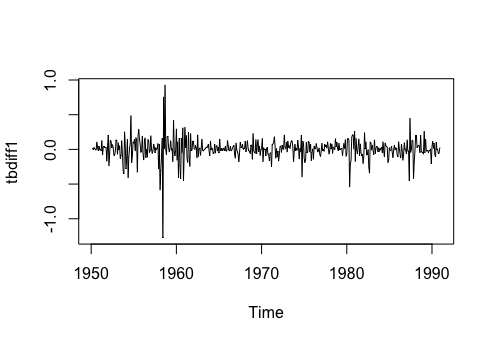
\includegraphics[width=0.5\linewidth]{mishk2.png}
    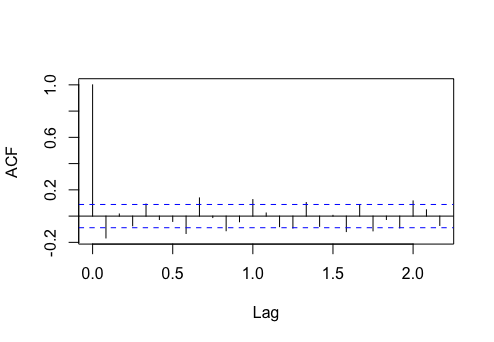
\includegraphics[width=0.5\linewidth]{mishk3.png}
\end{figure}

Podemos observar en el gráfico que la serie parece que presenta menos volatilidad a pesar del pico que aparece sobre los años 1959 - 1960. Además, no parece haber tendencia y la media parece ser constante a lo largo del tiempo. Fijándonos ahora en el gráfico ACF, vemos que aunque no decrece, muestra niveles más bajos de correlación que en el caso anterior. Todo esto nos indica que nuestra serie temporal transformada es débilmente estacionaria. \\

Para reafirmar nuestras conclusiones sobre los gráficos hacemos una prueba Dickey-Fuller de nuestra serie transformada. Recordamos que esta prueba busca la existencia de raíces unitarias en una serie temporal. 
\begin{lstlisting}[language=R]
> adf.test(tbdiff1)
p-value = 0.01
alternative hypothesis: stationary
\end{lstlisting}
Vemos que el p-valor obtenido en la prueba es menor que el nivel de significancia (0,05) y por lo tanto rechazamos la hipótesis nula. De esta manera vemos que nuestra conclusión es correcta y que necesitamos transformar la serie una vez para que ésta sea estacionaria. \\


Usando la función \texttt{auto.arima} para determinar los modelos $ARIMA$ no estacionales que mejor se ajustan, obtenemos en el AIC un modelo $ARIMA(3,1,5)$ y en el BIC un modelo $ARIMA(0,1,1)$. \\

Como podemos ver, para ambos criterios obtenemos que el modelo que mejor se ajusta tiene un orden de diferenciación igual a 1, ahora hacemos un test para ver si los coeficientes son estadisticamente significativos. Observamos que en el modelo AIC nos encontramos que los dos últimos coeficientes y el drift no son significativos, por lo tanto podemos considerar que son 0, de esta forma consideramos el modelo $ARIMA(3,1,3)$ y obtenemos un modelo con dos variables menos y un AIC más negativo, por lo tanto, es mejor que el $ARIMA(3,1,5)$. \\

Por último, examinamos los residuos de los dos modelos que hemos elegido para determinar qué modelo se ajustará mejor a nuestros datos. Los residuos estan definidos como $e_t=Y_t-\hat{Y}_t$, donde $\{Y_t\}_t$ es la serie temporal y $\hat{\{Y_t\}}_t$ es el modelo que hemos elegido para modelar la serie. Si el modelo es un buen ajuste, los residuos deberían comportarse como $WN(0,\sigma^2_\varepsilon)$.\\

\begin{figure}[H]
    \centering
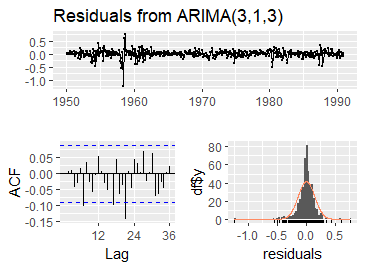
\includegraphics[scale=0.8]{Residuals from ARIMA(3,1,3).png}
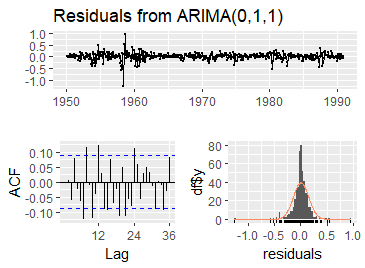
\includegraphics[scale=0.8]{Residuals from ARIMA(0,1,1).png}
\end{figure}

Como podemos ver, los residuos no están significativamente correlacionados entre ellos para ninguno de los modelos. Podemos pensar que tal vez para $ARIMA(0,0,1)$ sean un poco más grandes que para $ARIMA(3,1,5)$. Para comprobar este hecho realizaremos la prueba Ljung-Box para ambos modelos. La prueba Ljung-Box comprueba si la serie temporal tiene autocorrelación, siendo la hipótesis nula que los residuos estan distribuidos de manera independiente. \\

Realizaremos la prueba para ambos modelos durante los primeros 100 lags:
\begin{lstlisting}[language=R]
> checkresiduals(aic_model2, lag=100)
data:  Residuals from ARIMA(3,1,3)
p-value = 0.1691

> checkresiduals(bic_model, lag=100)
data:  Residuals from ARIMA(0,1,1)
p-value = 1.751e-06
\end{lstlisting}


Una vez hecha la prueba en ambos modelos, vemos que en el modelo $ARIMA(0,1,1)$ los datos no se distribuyen de forma independiente ya que rechazamos la hipótesis nula debido a que el p-valor=$1,751 \cdot e^{-6}<0,05$. En cambio en el modelo $ARIMA(3,1,3)$ no podemos rechazar la hipótesis nula ya que el p-valor es mayor que 0,05, por lo tanto podemos decir que los datos se distribuyen de forma independiente (es decir, las correlaciones en la población de la que se toma la muestra son 0, de modo que cualquier correlación observada en los datos es el resultado de la aleatoriedad del proceso de muestreo). De esta manera decidimos quedarnos con el modelo $ARIMA(3,1,3)$. Finalmente, nos quedamos con este último modelo devido a que el p-valor que obtenemos muestra que los residuos se distribuien independientemente $(<0.05)$ y por lo tanto, el modelo es correcto.



\end{document}